\documentclass[11pt, a4paper]{article}

% To automatically save paper and trees (at least, for preprints):
\usepackage{fullpage} % or \usepackage[headings]{fullpage}

%% FOR DRAFTS:
%\usepackage{color}
%\newcommand{\rojo}[1]{\textcolor{red}{#1}}

% To load external graphics:
%\usepackage{graphicx}
\usepackage{tikz}

% AMS packages, very recommended for maths:
\usepackage{amsmath, amsthm, amsfonts, amssymb}

\newtheorem*{theo}{Theorem}

% To automatically include internal hyperlinks 
% and internet links with \url{http://....} 
%\usepackage{hyperref}
%% DOI: https://doi.org/10.1080/00255572.2025.2588249

% Article no.~110.55
\title{The number $e$ as the limit of the solutions of a family of equations%
\footnote{\textbf{This paper has been published in} \textit{The Mathematical Gazette} \textbf{110} (2026), no.~579, 605--608, doi: 10.1080/00255572.2025.2588249.}}
\author{Juan Luis Varona\\[4pt]
\small Departamento de Matem\'aticas y Computaci\'on,\\[-1pt]
\small Universidad de La Rioja,\\[-1pt]
\small Logro\~no, Spain\\[2pt]
\small \texttt{jvarona@unirioja.es}\\[2pt]
\small ORCID: {0000-0002-2023-9946}}
\date{}     % Activate to display a given date or no date

\begin{document}

\maketitle

In a first-year university course on mathematical analysis, the number $e$, defined as
\[
e = \lim_{n\to\infty} \Big(1+\frac{1}{n}\Big)^n
\qquad \text{or} \qquad
e = \sum_{n=0}^{\infty} \frac{1}{n!},
\]
appears everywhere. But, why $e$ instead of another number? 
Of course, the main reason is that it is the basis of the exponential function, whose derivative is itself; however, it is still important to note that $e$ is a very special number, which has nice properties and characteristics, such as the one we are going to show here. Specifically, we demonstrate that the number $e$ can be defined as the limit of the solutions of a certain family of equations that answer a natural question.

Let us start by recalling that the Catalan conjecture (that was proved by Preda Mih\u{a}lescu in 2002) states that, for integers greater than $1$, the unique solution of $a^b - c^d = 1$ is $3^2 - 2^3 = 1$.

Although this is not requested by the conjecture, the solution has the form $(x+1)^x - x^{x+1} = 1$, which is particularly appealing. If we no longer consider integers but real numbers, which is greater, $(x+1)^x$ or $x^{x+1}$? 
% One might think that there will be an $x$ at which the inequality is reversed, 
% and mathematical intuition suggests that this may have something to do with the number~$e$.
Contrary to what happens in Catalan's solution, $x^{x+1}$ is greater for sufficiently large $x$, so there must be (at least one) $x$ for which the inequality is reversed, and mathematical intuition suggests that this may have something to do with the number~$e$.

There is no way to solve $(x+1)^x = x^{x+1}$ exactly, but numerically the solution is $x = 2.29317\dots$ Wow, it's not~$e$.
This can be seen in Figure~\ref{fig1}.
\begin{figure}[ht]
\centering
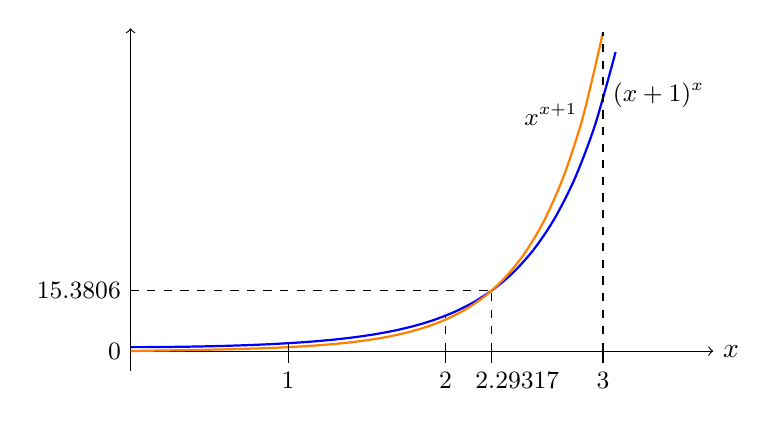
\begin{tikzpicture}[xscale=2,yscale=0.05]
    % Ejes
    \draw[->] (0,0) -- (3.7,0) node[right] {$\small x$};
    \draw[->] (0,-5) -- (0,82); % node[above] {$y$};

    % Curva y = (x+1)^x usando math expression
    \draw[domain=0.001:3.08,smooth,variable=\x,blue,thick]
        plot ({\x},{(\x+1)^\x});
    % Curva y = x^(x+1) usando math expression
    \draw[domain=0.001:3,smooth,variable=\x,orange,thick]
        plot ({\x},{\x^(\x+1)});

    \draw (0,0) node[left]{\small $0$};
%    %% x = 1.5;
%    %% FindRoot[(x + 1)^x == x^(x + 1), {x, 2}]
%    %% gives x = 2.29317
%    %% (x + 1)^x /. x -> 2.293166287411861
%    %% gives 15.3806
    \draw (2.29317,-3) node[below] {\small \qquad $2.29317$} -- (2.29317,0);
    \draw[dashed] (2.29317,0) -- (2.29317,15.3806);
    \draw[dashed] (0,15.3806) node[left]{\small $15.3806$} -- (2.29317,15.3806);
    \draw (1,-3) node[below] {\small $1$} -- (1,2);
    \draw (2,-3) node[below] {\small $2$} -- (2,0);
    \draw[dashed] (2,0) -- (2,9);
    \draw (3,-3) node[below] {\small $3$} -- (3,0);
    \draw[dashed] (3,0) -- (3,81);

    % Etiqueta
    \node[left] at (2.9,60) {\small $x^{x+1}$};
    \node[right] at (3,65) {\small $(x+1)^x$};
\end{tikzpicture}
\caption{The intersection of the curves $y=(x+1)^{x}$ and $y=x^{x+1}$.}
\label{fig1}
\end{figure}

What if, instead of $x$ and $x+1$, we use closer numbers?

The solution to $(x+1/2)^x = x^{x+1/2}$ is $x = 2.48733\dots$,
and the solution to $(x+1/3)^x = x^{x+1/3}$ is $x = 2.56011\dots$
We can try more numbers of the form $x$ and $x+1/n$ and, for example, the solution to $(x+1/1000)^x = x^{x+1/1000}$ is $2.71778\dots$ It seems that we are getting closer to~$e$. Is it true that the solution of $(x+1/n)^x = x^{x+1/n}$ tends to $e$ when $n$ tends to infinity?

What happens is as follows. Here we write $t = 1/n$ and study the limit as $t \to 0^{+}$, which is equivalent to the previous question. And, for the sake of completeness, 
we also analyse the case $t \to 0^{-}$, and the behavior of the solutions when $t \to \pm \infty$.
%% Analyze is predominantly used in American (US) English
%% Analyse is predominantly used in British English

\begin{theo}
For every nonzero real number $t$, the equation $(x+t)^x = x^{x+t}$ has a unique real solution. If we denote that solution by $x(t)$, then $\lim_{t\to0} x(t) = e$.
Moreover, $\lim_{t\to\infty} x(t) = 1$, and $\lim_{t\to-\infty} (x(t)+t) = 1$ (i.e., $x(t) \sim 1-t$ asymptotically when $t\to-\infty$).
\end{theo}

\begin{proof}
Let us note that
\[
(x+t)^x = x^{x+t} 
\iff
x\log(x+t) = (x+t)\log(x)
\iff 
\frac{\log(x)}{x} = \frac{\log(x+t)}{x+t}.
\]
Moreover, if we take $f(x) = \log(x)/x$, then $f'(x) = (1-\log(x))/x^2$, 
so $f(x)$ increases in $(0,e)$ and decreases in $(e,\infty)$, and $x=e$ is a maximum.

Now, let us consider the case $t>0$. Then, the proofs of $\lim_{t\to\infty} x(t) = 1$ and $\lim_{t\to0^+} x(t) = e$ are clear when observing Figure~\ref{fig2}, which, for fixed $t>0$, illustrates the solution of $f(x)=f(x+t)$. Let's look at the increasing and decreasing parts of the function $f$. The horizontal distance $t$ between the two points that have the same height above the horizontal axis (that is, $f(x)=f(x+t)$) decreases continuously as the height increases. When the height is close to~$0$ (which occurs when $x$ is close to~$1$), the distance $t$ is close to~$\infty$; and, as we approach the maximum of $f$, which is at $e$, the distance $t$ tends to~$0$.
\begin{figure}[ht]
\centering
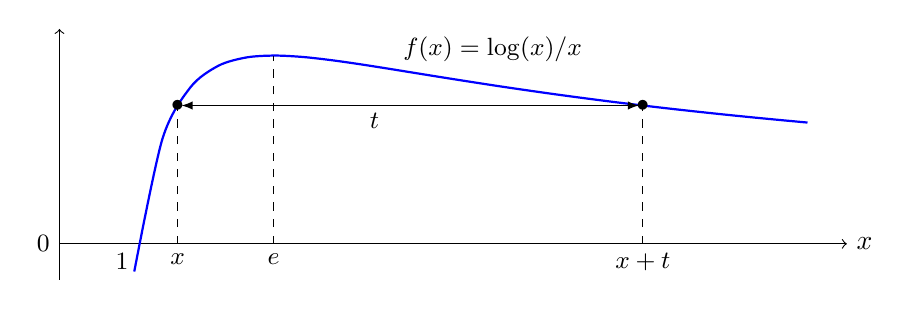
\begin{tikzpicture}[xscale=1,yscale=6.5]
    % Ejes
    \draw[->] (0,0) -- (10,0) node[right] {$\small x$};
    \draw[->] (0,-0.07) -- (0,0.42); % node[above] {$y$};

    % Curva y = ln(x)/x usando math expression
    \draw[domain=0.95:9.5,smooth,variable=\x,blue,thick]
        plot ({\x},{ln(\x)/\x});
    
    \draw (0,0) node[left]{\small $0$};
    \draw (1,0) node[below left]{\small $1$};
    \draw[dashed] (2.71828,0) node[below]{\small $e$} -- (2.71828,0.367879);
    %% x = 1.5;
    %% FindRoot[Log[x]/x == Log[xmast]/(xmast), {xmast, 7.5}]
    %% gives xmast = 7.40876
    \draw (1.5,{ln(1.5)/1.5}) node{\small $\bullet$}; 
    \draw (7.40876,{ln(7.40876)/7.40876}) node{\small $\bullet$}; 
    \draw[latex-latex] (1.5+0.05,{ln(1.5)/1.5}) -- (7.40876-0.05,{ln(7.40876)/7.40876}); 
    \draw[dashed] (1.5,0) node[below]{\small $x$} -- (1.5,{ln(1.5)/1.5});
    \draw[dashed] (7.40876,0) node[below]{\small $x+t$} -- (7.40876,{ln(7.40876)/7.40876});
    \draw (4,0.24) node{\small $t$};

    % Etiqueta
    \node at (5.5,0.38) {\small $f(x) = \log(x)/x$};
\end{tikzpicture}
\caption{For fixed $t>0$, the solution of $f(x)=f(x+t)$.}
\label{fig2}
\end{figure}

For $t<0$, take $u=-t$ and $y = x+t$. Then the equation $(x+t)^x = x^{x+t}$ becomes $y^{y+u} = (y+u)^y$ with $u>0$, so we are in the previous case, and the result follows.
\end{proof}

Notice that, in particular, this shows that the number $e$ can be defined as the limit of the solutions of the equations $(x+1/n)^x = x^{x+1/n}$ when $n\to \infty$.

\paragraph{Funding.} This research was partially supported by PID2024-155593NB-C22 (Mi\-nis\-te\-rio de Cien\-cia, Inno\-va\-ci\'on y Uni\-ver\-si\-da\-des, Spain)

\paragraph{Disclosure statement.} No potential conflict of interest was reported by the author.

\end{document}


